\documentclass[12pt]{report}
\title{Mid Term Project}
\usepackage{amsmath}
%\usepackage{maplestd2e}
\usepackage{tikz}
\usetikzlibrary{arrows.meta,shapes.misc,patterns,shapes.symbols,decorations.pathreplacing,decorations}
\usepackage{amssymb}
\AtBeginDocument{\renewcommand{\chaptername}{}}
\usepackage{microtype}
\usepackage[bottom=30 mm, top=25 mm, left=25 mm, right=25 mm]{geometry}
\usepackage{multicol}
\usepackage{titlesec} 
\usepackage{graphicx}
\usepackage{listings}
\usepackage{xcolor}
\usepackage{amsmath}
\usepackage{subfigure}
\usepackage{subfig}
\usepackage{wasysym}
\usepackage{mathtools}
\usepackage{wrapfig}
\usepackage{float}
\usepackage{lipsum} 
%\usepackage[framed,numbered,autolinebreaks,useliterate]{mcode}
\lstset{
    breaklines=true,
    tabsize=3,
    showstringspaces=false
}

\lstdefinestyle{Common}
{
    extendedchars=\true,
    language={[Visual]Basic},
    frame=single,
    framesep=3pt,
    framerule=0.4pt,
    xleftmargin=3.4pt,
    xrightmargin=3.4pt,
    rulecolor=\color{red}
}

\lstdefinestyle{A}
{
    style=Common,
    backgroundcolor=\color{yellow!10},
    basicstyle=\scriptsize\color{black}\ttfamily,
    keywordstyle=\color{black},
    identifierstyle=\color{black},
    stringstyle=\color{red},
    commentstyle=\color{black}
}

\makeatletter 
\renewcommand\chapter{\thispagestyle{plain}%
\global\@topnum\z@
\@afterindentfalse
\secdef\@chapter\@schapter}
\makeatother 

\titleformat{\chapter}{\bfseries\Huge}{\thechapter.\quad}{0em}{}


\usepackage[utf8]{inputenc}
\parindent0pt

\begin{document}

%\setlength{\parindent}{3ex} 

\begin{large}

\thispagestyle{empty}
\begin{center}
\begin{figure}[t]
\centering
%
\includegraphics[scale=0.52]{sdsu_logo.png}
\end{figure}
\end{center}
\begin{center}
\Large{Department of Mathematics and Statistics}
\end{center}
\begin{center}
\Large{Prof. Joseph Mahaffy}
\end{center}
\begin{center}
\Large{Math 636, Mathematical Modeling}
\end{center}
\begin{verbatim}



\end{verbatim}
\begin{center}
\textbf{\Huge{Homework Assignment}}
\end{center}
\begin{verbatim}


\end{verbatim}
\rule{16,5 cm}{0.4pt}\\
\begin{center}
\textbf{\LARGE{Stochastic Modeling}}\\[0,7 cm]
\end{center}
\rule{16,5 cm}{0.4pt}
\begin{verbatim}


\end{verbatim}

\begin{center}
 \textbf{by Matteo Polimeno} \\ 
\textbf{12/5/2017}\\

\end{center}
\end{large}


\newpage

%\tableofcontents
\newpage

\sloppy

\newpage


\chapter{Problem 1}
The transition matrix for red squirrels, gray squirrels, both or neither in that order is given by
\begin{align*}
T  &= \begin{bmatrix}
    0.8797 & 0.0382 & 0.0527 & 0.0008 \\
    0.0212 & 0.8002 & 0.0041& 0.0143 \\
    0.0981 & 0.0273 & 0.8802 & 0.0527\\
    0.0010 & 0.1343 & 0.0630 & 0.9322
 	  \end{bmatrix}
\end{align*}

The equilibrium distribution of squirrels based on this transition matrix is given by the normalized eigenvector associated with the eigenvalue $\lambda=1$, which is found to be
\begin{align*}
    \textbf{$x_{e}$} &= \begin{bmatrix}
           0.1705 \\
           0.0560 \\
           0.3421 \\
           0.4313
         \end{bmatrix}
\end{align*}

This eigenvector shows that the predicted squirrel community for the given region of the Great Britain should be approximately 17\% red squirrels, 6\% grey squirrels, 34\% both and 43\% neither. Therefore the native red squirrel, which starts off as being 87\% of the total squirrel population, will end up being 17\%, while the grey squirrel goes from 2\% to 6\%. Interestingly, the total population at the equilibrium will be made of 43\% different species of squirrels, whereas at $t=0$ those were only 0.1\% of the total.\\
Therefore, this model seems to suggest that the invasive grey species will displace the native red squirrel, however the latter will not go extinct nor will be outnumbered by the invasive grey squirrel, as we can see that, there is going to be a higher overall percentage of red squirrels anyway at the equilibrium distribution.

\chapter{Problem 2}
\section{Part a}
From the transition model given, knowing that 100 frogs were released in the first habitat at $t=0$, we find the expected distribution of the tagged frogs after 1,2,5 and 10 days to be, respectively
\begin{align*}                                     \textbf{$D_{1}$} = \begin{bmatrix} 
42\\
7 \\
34 \\
17
\end{bmatrix},\
\textbf{$D_{2}$} = \begin{bmatrix}
27.94 \\
15.97 \\
37.54 \\
18.55
\end{bmatrix},\
\textbf{$D_{5}$} = \begin{bmatrix}
23.1737 \\
20.6571 \\
35.6359 \\
20.5333
\end{bmatrix},\
\textbf{$D_{10}$} = \begin{bmatrix}
23.0600 \\
20.6914\\
35.4725\\
20.7762
\end{bmatrix}
\end{align*}

\section{Part b}
The expected distribution after a long period of time is given by the following normalized eigenvector of the eigenvalue $\lambda=1$
\begin{align*}
    \textbf{$D_{long}$} &= \begin{bmatrix}
           23.06 \\
           20.69 \\
           35.47\\
           20.78
         \end{bmatrix},
\end{align*}
which means that, after a long period of time, about 23\% of the frogs will be living in the first habitat, around 20.7\% will be leaving on the second habitat, a little over 35\% will be living in the third habitat and around 20.8\% will be leaving in the fourth habitat. Now, as we started with 100 frogs and obviously we can't have fractionary animals, we can approximate and say that, according to our simulation, 23 frogs will be living in the first habitat, 21 in the second habitat, 35 in the third and 21 in the fourth. \\
At a first glance, just by looking at the distribution above, it seems to be that the third habitat is the most suitable for the frogs, as a higher percentage of them will tend to move over there as time goes on, whereas the fourth and second habitats seem to be least suitable as they are the least populated by the frogs after a long period of time.\\
However, it seems reasonable to conclude that the least suitable habitat for the frogs is the first one. In fact, it's the one from which most frogs leave as time proceeds, going from 42 after the first day to around 23 after a long period of time, which seems to suggest that frogs do not find such habitat to be suitable for them and tend to leave from it. Whereas, the second and the fourth habitat increase their number of frogs up until roughly 21, and then keep it that way as time goes on.\\
Also, the third habitat seems to be the most stable one in terms of distribution of frogs, which seems to oscillate between 37 and 35 of the total.\\
If we compare these results with our observations in Part a, we can see that the trend was clear already after the first day, and in fact the distribution of frogs among the habitats found after a long period of time is very much similar to the distribution found after 10 days.
\section{Part c}
Below is the Matlab code implemented to run a MonteCarlo simulation of this experiment run 1000 times.
\begin{lstlisting}[style=A]
co%Monte Carlo Simulation for Problem 2, Part c

%Distribution matrix for the frogs population (not necessary, but listed to
%see what data we are working with)
bratakoi = [0.42 0.16 0.19 0.16;
0.07 0.38 0.24 0.13;
0.34 0.19 0.51 0.27;
0.17 0.27 0.06 0.44]; 

count1 = zeros(10,1000); %initializing frogs count
count2 = zeros(10,1000);
count3 = zeros(10,1000);
count4 = zeros(10,1000);

btk = ones(1000,100,10); %initializing and setting all 100 frogs in 
%habitat 1 for 10 days and 1000 simulations

for k = 1:10 %number of days 
for j = 1:1000 %number of simulation
for i = 1:100 %each individual frog goes through loop
if btk(j,i,k) == 1 %if frog is in habitat 1, function hbt_1
btk(j,i,k) = hbt_1; %all frogs released in habitat 1 
%go through this function when k=1 
elseif btk(j,i,k) == 2 %if frog is in habitat 2, function hbt_2
btk(j,i,k) = hbt_2; %kicks in when k=2
elseif btk(j,i,k) == 3 
btk(j,i,k) = hbt_3; %same 
else 
btk(j,i,k) = hbt_4; %same
end

if btk(j,i,k) == 1 %counts # of frogs that ends up in which habitat
count1(k,j) = count1(k,j)+1; 
elseif btk(j,i,k) == 2
count2(k,j) = count2(k,j)+1;
elseif btk(j,i,k) == 3
count3(k,j) = count3(k,j)+1;
else
count4(k,j) = count4(k,j)+1;
end
end   
end
btk(:,:,k+1) = btk(:,:,k); %sets the next day simulation to start with previous
end

%array btk ends up being 10 arrays, one per day, of where the 100 frogs end
%up. Individual frogs are the columns, number of simulations are the rows.

mean1 = [mean(count1(1,:)) mean(count2(1,:))... %Distribution vector 
mean(count3(1,:)) mean(count4(1,:))]'/100;  %with mean of frogs per habitat of day 1.

std1 = [std(count1(1,:)) std(count2(1,:))...  %Std deviation
std(count3(1,:)) std(count4(1,:))]'/100;  %of frogs per habitat of day 1.

mean2 = [mean(count1(2,:)) mean(count2(2,:))... %Same for day 2.
mean(count3(2,:)) mean(count4(2,:))]'/100;
std2 = [std(count1(2,:)) std(count2(2,:))...
std(count3(2,:)) std(count4(2,:))]'/100;

mean3 = [mean(count1(5,:)) mean(count2(5,:))... %Day 5.
mean(count3(5,:)) mean(count4(5,:))]'/100;
std3 = [std(count1(5,:)) std(count2(5,:))...
std(count3(5,:)) std(count4(5,:))]'/100;

mean4 = [mean(count1(10,:)) mean(count2(10,:))... %Day 10.
mean(count3(10,:)) mean(count4(10,:))]'/100;
std4 = [std(count1(10,:)) std(count2(10,:))...
std(count3(10,:)) std(count4(10,:))]'/100;
\end{lstlisting}

The following are the means and standards deviation for the distribution of the frogs after 1,2,5 and 10 days respectively
\begin{align*}
    \textbf{$\mu_{1}$} = \begin{bmatrix}
           43.0870 \\
           6.8770\\
           33.9890\\
           16.0470
         \end{bmatrix},\
    \textbf{$\sigma_{1}$} = \begin{bmatrix}
           4.8260\\
           2.5535\\
           4.6539\\
           3.7639
         \end{bmatrix},
\end{align*}
\begin{align*}
    \textbf{$\mu_{2}$} = \begin{bmatrix}
           29.0390 \\
           15.9640\\
           37.6650\\
           17.3320
         \end{bmatrix},\
    \textbf{$\sigma_{2}$} = \begin{bmatrix}
           4.6044\\
           3.5422\\
           4.9080\\
           3.8197
         \end{bmatrix},
\end{align*}
\begin{align*}
    \textbf{$\mu_{5}$} = \begin{bmatrix}
           24.3480 \\
           20.6410\\
           35.8830\\
           19.1280
         \end{bmatrix},\
    \textbf{$\sigma_{5}$} = \begin{bmatrix}
           4.2866\\
           4.1409\\
           4.9762\\
           3.8772
         \end{bmatrix},
\end{align*}
\begin{align*}
    \textbf{$\mu_{10}$} = \begin{bmatrix}
           24.4670 \\
           20.5220\\
           35.7660\\
           19.2450
         \end{bmatrix},\
    \textbf{$\sigma_{10}$} = \begin{bmatrix}
           4.4979\\
           4.0007\\
           4.8298\\
           3.7645
         \end{bmatrix}.
\end{align*}

As we can see, the mean values obtained with the Monte Carlo simulation are all within the standard devation, if compared to our previous results from Part a.

\chapter{Problem 3}
\section{Part a}
$P_{n}$ is a vector that varies discretely with time. Let $L$ be our Leslie Matrix with $P_{n} = [P_{1}, P_{2}, P_{3}, P_{4}]_{n}^{T}$ the population vector at time $n$ divided in 4 age classes (0-1,1-2,2-3,3-4). Then the Leslie Model is
$$
P_{n+1}=LP_{n},
$$
where $L$ is our Leslie matrix defined as
\begin{align}
L  &= \begin{bmatrix}
0 & 1.5 & 2.2 & 3.4 \\
0.4 & 0 & 0 & 0 \\
0 & 0.7 & 0 & 0\\
0 & 0 & 0.75 & 0
\end{bmatrix}.
\end{align}
To find the steady-state percentage for each age group with build a model and run it. The dominant eigenvalue is found to be $\lambda$=1.2465, which implies that the population growth is about 25\% over a 1-year period. The associated eigenvector is found to be\\
\begin{align}
\textbf{$P_{e}$} &= \begin{bmatrix}
0.6213\\
0.1994\\
0.1120\\
0.0674
\end{bmatrix},
\end{align}
this shows that the steady-state distribution should be approximately 62\% in the 0-1 age group, about 20\% in the 1-2 age group, about 11\% in the 2-3 age group and finally a little less than 7\% in the 3-4 age group.\\
The time that it takes for the population to double after reaching its steady-state distribution is found to be
$$
t=3.1460,
$$
thus this population, according to this model, will double in size after roughly 3 years and two months.

\section{Part b}
The survival rates $s_{2}$ and $s_{4}$ is reduced by a fraction $\alpha$, so that the survival rate of 1-2 years old is 0.7$\alpha$ and the survival rate of 2-3 years old is 0.75$\alpha$. We compute the value of $\alpha$ in MatLab and we find it to be
$$
\alpha = 0.4324.
$$
Then, for this value of $\alpha$ and 550 mature (3-4 years old) animals, we determine the total population to be
$$
P_{tot} = 20066,
$$
whereas the population for each age group is found to be
\begin{align}
\textbf{$P_{e}$} &= \begin{bmatrix}
12860\\
5144\\
1557\\
505
\end{bmatrix}.
\end{align}
As for the total number of animals harvested each year under this conditions, this is found to be roughly equal to 834.

\chapter{Problem 4}
\section{Part a}
Using the data and information given, we found the average survival rates $s_{12}$, $s_{23}$ and $s_{33}$ to be
$$
s_{12} = 0.3564,
$$
$$
s_{23} = 0.7339 = s_{33}.
$$

As for the average birth rates $b_{2}$ and $b_{3}$ we found
$$
b_{2} = 0.8118,
$$
$$
b_{3} = 2.0038.
$$

\section{Part b}
From the results found in Part a, we can build the following Leslie matrix
\begin{align}
L  &= \begin{bmatrix}
0 & 0.8118 & 2.0038\\
0.3564 & 0 & 0\\
0 & 0.7339 & 0.7339
\end{bmatrix}.
\end{align}

Using this matrix we found the population for each of the age classes over the next three years and the following are results in vector form starting with the population after 1 year

\begin{align}
\textbf{$P_{1}$} &= \begin{bmatrix}
365.2366\\
110.8404\\
173.9343
\end{bmatrix},
\end{align}

so the population for the first age group (0-1 years old) after one year will be about 365 birds, for the second age group (1-2 years old) will be about 111 birds and for the third group (older than 2 years old) will be about 174 birds.\\
Now the population vector for the distribution after 2 years

\begin{align}
\textbf{$P_{2}$} &= \begin{bmatrix}
438.5098\\
130.1703\\
208.9962
\end{bmatrix},
\end{align}

so the population for the first age group (0-1 years old) after two years will be about 439 birds, for the second age group (1-2 years old) will be about 130 birds and for the third group (older than 2 years old) will be about 209 birds.\\

Now the population vector for the distribution after 3 years

\begin{align}
\textbf{$P_{3}$} &= \begin{bmatrix}
524.4588\\
156.2849\\
248.9143
\end{bmatrix},
\end{align}

so the population for the first age group (0-1 years old) after two years will be about 524 birds, for the second age group (1-2 years old) will be about 156 birds and for the third group (older than 2 years old) will be about 249 birds.\\

\section{Part c}
The eigenvvalues for the model are found to be
$$
\lambda_{1} = -0.2303 + 0.4560i,
$$
$$
\lambda_{2} = -0.2303 - 0.4560i,
$$
$$
\lambda_{3} = 1.1946,
$$

so we have a pair of complex conjugates (both with negative real part) and a real positive eigenvalue, which is the dominant one.\\
The eigenvectors for $\lambda_{1}$, $\lambda_{2}$ and $\lambda_{3}$, respectively, are found to be
\begin{align*}                                     \textbf{$V_{1}$} = \begin{bmatrix} 
0.7631\\
-0.2400 - 0.4752i \\
0.0095 + 0.3662i
\end{bmatrix},\
\textbf{$V_{2}$} = \begin{bmatrix}
0.7631 \\
-0.2400 + 0.4752i \\
0.0095 - 0.3662i
\end{bmatrix},\
\textbf{$V_{3}$} = \begin{bmatrix}
0.8721 \\
0.2602 \\
0.4145
\end{bmatrix}.
\end{align*}
The limiting age population in each of the age classes is found to be
\begin{align*}                                     \textbf{$P_{e}$} = \begin{bmatrix} 
0.5638\\
0.1682\\
0.2680
\end{bmatrix}.
\end{align*}
Therefore, given our dominant eigenvalue of $\lambda_{3} = 1.1946$, we see that, once the population reaches this limiting distribution, the approximate annual growth rate is 19\%.\\
To find the time that it takes for the population to double we simply compute
$$
\frac{\log(2)}{1.1946} = 3.8985,
$$
therefore the population doubles after roughly 3 years and 11 months.

\chapter{Problem 5}
\section{Part a}
Michaelis-Menten enzymes follow simple first order kinetics, i.e. the rate of the reaction depends only on  one of the reactants, the substrate. If we let $S_{1}$ be the substrate, $S_{2}$ be the enzyme, $S_{3}$ be the enzyme-substrate complex and $S_{4}$ be the resultant product, then we can write a chemical reaction for the transformation of $S_{1}$ in  $S_{4}$ as\\

$S_{1}$ + $S_{2}$  $\xrightarrow{\mbox{\tiny{$c_{1}$}}} S_{3}$\\


$S_{3}$ $\xrightarrow{\mbox{\tiny{$c_{2}$}}} S_{1} + S_{2}$\\


$S_{3}$ $\xrightarrow{\mbox{\tiny{$c_{3}$}}} S_{2} + S_{4}$,\\

where $c_{1}$, $c_{2}$, $c_{3}$ are the rate constants for each reaction.\\
Let a cell of \textit{E.Coli} have $S_{1}$=500 molecules of substrate, $S_{2}$=50 molecules of enzyme and $S_{3}=S_{4}=0$, when the reaction begins. The rate constants satisfy:
$$
c_{1} = 0.002, c_{2} = 6 \cdot 10^{-5}, c_{3} = 0.08.
$$
We develop a Gillespie Algorithm for these Michaelis-Menten enzyme reactions and present 2 distinct simulations of the time series for $t \in [0,200]$, using the same rate constants listed above. Below is the code built \newpage
\begin{lstlisting}[style=A]
% LV_gill.M
% Simple implementation of the Stochastic Simulation Algorithm
% (or Gillespie's algorithm) for the Lotka-Volterra system.
%
% rand('state',100) % Can fix rand # pattern
% stoichiometric matrix for rxs
V = [-1 1 0;-1 1 1;1 -1 -1;0 0 1];
%%%%%%% Parameters and Initial Conditions
X = zeros(4,1);
X(1) = 500;   % initial molecules of S1 (substrate)
X(2) = 50;   % initial molecules of S2 (enzyme)
X(3) = 0;   % initial molecules of S3 (enzyme-substrate complex)
X(4) = 0;   % initial molecule of S4 (product)

Y1(1) = X(1);  % store # of molecules
Y2(1) = X(2);
Y3(1) = X(3);
Y4(1) = X(4);

% set chem rx coefficients
c(1) = 0.002; c(2) = 0.00006; c(3) = 0.08;
t = 0;         % initial time
T(1) = t;
tfinal = 200;   % final time
i = 1;
while t < tfinal
% rx combination functions
a(1) = c(1)*X(1)*X(2);
a(2) = c(2)*X(3);
a(3) = c(3)*X(3);
asum = sum(a);  % total a
% generate rand # and find rx occurring
j = min(find(rand<cumsum(a/asum)));
% 2nd rand # for time until rx
tau = log(1/rand)/asum;
X = X + V(:,j); % Stochastic matrix adjusts X
t = t + tau;
i = i + 1;
T(i) = t;
Y1(i) = X(1);
Y2(i) = X(2);
Y3(i) = X(3);
Y4(i) = X(4);
figure(101)
plot(T,Y1,'b-',T,Y2,'r-',T,Y3,'m-',T,Y4,'g-');grid;
xlim([0,200]);
fontlabs = 'Times New Roman'; % Font type used in labels
xlabel('$t$','FontSize',14,'FontName',fontlabs,...
'interpreter','latex');  
ylabel('Molecules','FontSize',14,'FontName',fontlabs);  
set(gca,'FontSize',12);
legend('S1','S2','S3','S4','location','best');
title('Michaelis-Menten Enzyme Reactions using Gillespie Algorithm');
\end{lstlisting}


The following figure shows two different simulations of the time series $t \in [0,200]$ for all 4 chemical species

\begin{figure}[H]
	\subfigure[]{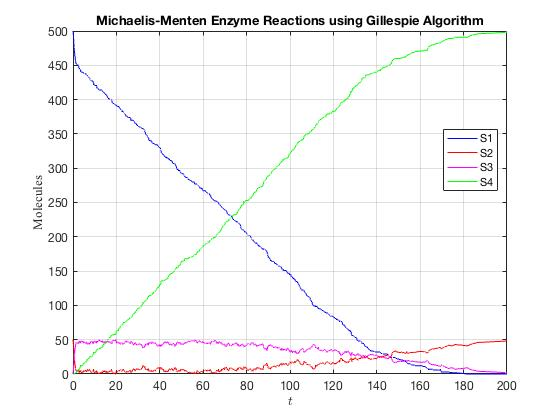
\includegraphics[scale=0.75]{Gillespie_Prob5a1.jpg}}
	\subfigure[]{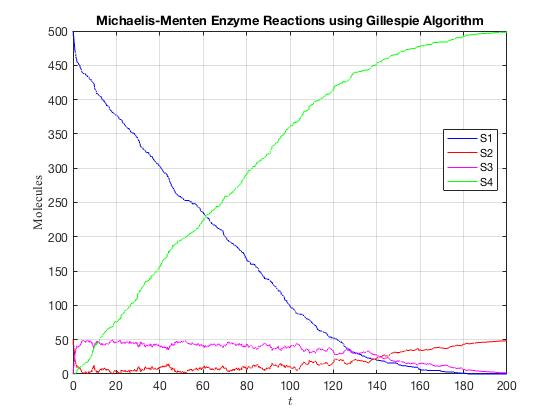
\includegraphics[scale=0.75]{Gillespie_Prob5a2.jpg}}
	\caption{a)First Simulation; b) Second Simulation}
\end{figure}

In Figure 5.1a we see that the concentration of the substrate $S_{1}$ (blue line) steadily decreases as time goes on, resembling an exponential decay, from its initial value of 500 molecules at $t=0$ to asymptotically approaching zero. The almost exact opposite "route" is followed by the product $S_{4}$,(green line) whose concentration that starts obviously at zero molecules and steadily increases, levelling off at around 500 molecules. The concentrations of the two chemical species crosses each other at around $t=70$.\\
As for the enzyme concentration $S_{2}$ (red line), it start at 50 molecules, almost instantaneously drops close to zero and seems to oscillate between zero and 10 molecules up until $t=80$, when it appears to more steadily increases all the way until $t=200$ when it comes back to 50 molecules. This is in accord with enzyme kinetics, as the enzyme regenerates after the formation of the product, getting ready to catalyse a new reaction. The enzyme-substrate complex follows almost exactly the opposite "route" of the enzyme, and we can see that its concentration $S_{3}$ (magenta line) starts at zero and almost immediately peaks at around 50 molecules, where it stays pretty much constant, with some minor fluctuations, up until $t=80$ when it seems to be more steadily decreasing up until $t=200$ when it reaches zero. The enzyme concentration and the enzyme-substrate complex concentration cross their paths at around $t=143$, and they cross the substrate concentration almost immediately after, the enzyme at $t=145$, while the enzyme-substrate complex at $t=150$ .\\
All of this is in accordance with what we know about enzyme kinetics, as the enzyme is regenerated at the end of the reaction and with the law of concentration of mass, as we start with a total of 550 molecules and we end up with a total of 550 and 50 molecules.\\

In Figure 5.1b we see that the concentration of the substrate $S_{1}$ (blue line) steadily decreases as time goes on, resembling an exponential decay, from its initial value of 500 molecules at $t=0$ to asymptotically approaching zero. The almost exact opposite "route" is followed by the product $S_{4}$,(green line) whose concentration that starts at zero molecules and then steadily increases to level off at around 500 molecules. The concentrations of the two chemical species cross each other at around $t=61$.\\
As for the enzyme concentration $S_{2}$ (red line), it start at 50 molecules, and drops close to zero at around $t=5$, then seems to oscillate between zero and 10 molecules up until $t=80$, when it appears to more steadily increases all the way until $t=200$ when it comes back to 50 molecules. This is in accord with enzyme kinetics, as the enzyme regenerates after the formation of the product, getting ready to catalyse a new reaction. The enzyme-substrate complex follows almost exactly the opposite "route" of the enzyme, and we can see that its concentration $S_{3}$ (magenta line) starts at zero and peaks at around 50 molecules at around $t=5$, then it stays pretty much constant, with some minor fluctuations, up until $t=80$ when it seems to be more steadily decreasing up until $t=200$ when it reaches zero. The enzyme concentration and the enzyme-substrate complex concentration cross their paths at around $t=143$, after having crossed the path of the concentration of the substrate, the enzyme at $t=139$, while the enzyme-substrate complex at $t=130$ respectively.\\
All of this is in accordance with what we know about enzyme kinetics, as the enzyme is regenerated at the end of the reaction and with the law of concentration of mass, as we start with a total of 550 molecules and we end up with a total of 550 and 50 molecules.\\
\section{Part b}
We can rewrite the reactions of Part a) as system of 4 differential equations, as follows
$$
\frac{d[S_{1}]}{dt} = -c_{1}[S_{1}][S_{2}] + c_{2}[S_{3}]
$$
$$
\frac{d[S_{2}]}{dt} = -c_{1}[S_{1}][S_{2}] + (c_{2}+c_{3})[S_{3}]
$$
$$
\frac{d[S_{3}]}{dt} = c_{1}[S_{1}][S_{2}] - (c_{2}+c_{3})[S_{3}]
$$
$$
\frac{d[S_{4}]}{dt}  = c_{3}[S_{3}],
$$
where $[S_{1}]$, $[S_{2}]$, $[S_{3}]$, $[S_{4}]$ are the concentration of the substrate, the enzyme, the enzyme-substrate complex and the product respectively.\\
The figure below shows a graph of the ODE simulation (Figure 5.2a) by itself and a graph of the ODE simulation overlayed with one from the Gillespie stochastic simulation algorithm for the same reactions.

\begin{figure}[H]
	\subfigure[]{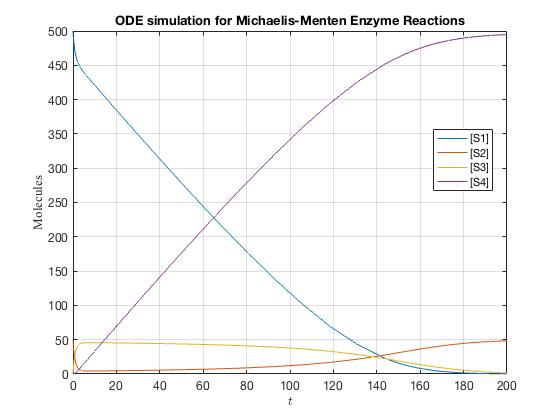
\includegraphics[scale=0.75]{Gillespie_Prob5b1.jpg}}
	\subfigure[]{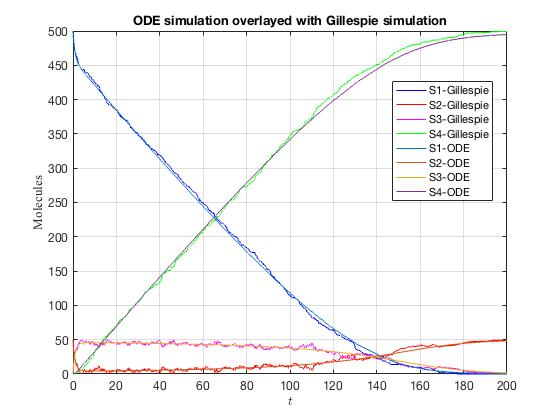
\includegraphics[scale=0.75]{Gillespie_Prob5b2.jpg}}
	\caption{a)ODE simulation; b) ODE vs. Gillespie Simulation}
\end{figure}

Figure 5.2 shows how the Gillespie Algorithm and the ODE simulation compare to each other. The overall trend appears to be basically the same, with the ODE simulation giving smoother graphs, whereas the Gillespie Algorithm has more "irregular" paths. Obviously the ODE simulation assume the reaction to be happening in a continuous manner, such that there are no corners or irregularities in the graphs, whereas the Gillespie Algorithm uses a stochastic approach and allows small fluctuations to happen among the concentrations of the different chemical species, giving, in this regard, a more realistic picture of the evolution of the reaction. In fact, it's unlikely that the concentration of the various species will just follow a smooth path from the beginning to the end of the reaction, as there are many factors that could alter the stability of the system at any given moment and the Gillespie Algorithm takes into account the different probabilities that the species interact with each other at any given moment.\\
That being said, both approaches give the same general trend for the overall reaction.

\section{Part c}
Using the quasi-steady state approximation, the Michaelis-Menten enzyme reactions can be re-written as the following system of differential equations
$$
\frac{ds_{1}}{dt} = - \frac{V_{m}s_{1}}{K_{m}+s_{1}}
$$
$$
\frac{ds_{4}}{dt} = \frac{V_{m}s_{1}}{K_{m}+s_{1}},
$$
where $s_{1}$ and $s_{4}$ are the concentration of the substrate and the product respectively, and $V_{m}$ and $K_{m}$ are kinetic constants.\\
So, our first estimate of the two parameters is done by applying some basic knowledge about Michaelis-Menten enzyme kinetics:
$$
V_{m} = c_{2}[S_{2}]_{t=0} \rightarrow  V_{m} = 4,
$$
$$
K_{m} = \frac{c_{2}+c_{3}}{c_{1}} \rightarrow K_{m} = 40.03,
$$
where $[S_{2}]$ is the concentration of the enzyme at the beginning of the reaction (i.e. 50 molecules in our case), and $c_{1}$, $c_{2}$, $c_{3}$ are the kinetic constants given in Part a.\\
So from here, we build a MatLab code to optimise $V_{m}$ and $K_{m}$ using fminsearch and we find the optimal values to be
$$
V_{m} = 4.8224,
$$
$$
K_{m} = 88.9313.
$$
The sum of square errors is found to be
$$
SSE =  12588
$$
Below is a graph for the simulations of the systems in Parts b and c 
\begin{figure}[H]
	\subfigure{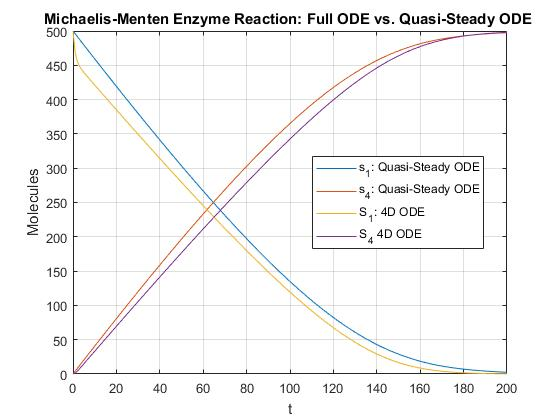
\includegraphics[scale=0.75]{Gillespie_Prob5c.jpg}}
	\caption{4D-ODE Simulation vs. Quasi-Steady State Simulation }
\end{figure}
Figure 5.3 shows that for both simulation the overall trend is the same, as the concentration on the product steadily decreases until it gets to zero (or very close to it), while the concentration of the product steadily increases until it gets to 500 (or very close to it), as expected.\\
However, a couple of differences can be noticed right away: first of all, according to the system build in Part b, the concentration of the product almost instantaneously drops from its starting value of 500 to 450 molecules, whereas in the quasi-steady state simulation the path of the substrate is smoother, with no abrupt drops. Interestingly, the substrate and the product cross each other at the same time in both simulation (around $t=70$), however, at that point in time, substrate and product have different concentrations in the two simulations: in the 4D-ODE simulation of Part b, when they intersect they both have around 225 molecules, whereas in the quasi-steady state simulation when they intersect they both have about 250 molecules, which corresponds to half the initial concentration of the substrate and half the final concentration of the product.\\
As for the product, both simulations have the same overall trend, but the quasi-steady state simulation shows a faster increase in its concentration if compared to the simulation run in Part b.

\section{Part d}
To convert from molecules to mole, we divide the number of molecules by the Avogadro number, which is given by
$$
N_{A} \approx 6.022 \cdot 10^{23} molecules/mole.
$$
We are given that the volume of the $\textit{E.Coli}$ is
$$
V = 7 \cdot 10^{-19}L
$$
Therefore the conversion from $\textit{molecules/E.Coli}$ to $\textit{Moles/Liter}$ is achieved by doing the following units multiplication
$$
\left(\frac{molecules}{E.coli} \cdot \frac{E.Coli/N_{A}}{7 \cdot 10^{-19}L}\right).
$$
So, since we start with 500 molecules of substrate [$S_{1}$], 50 of enzyme [$S_{2}$] and obviously zero of enzyme-substrate complex as well as product, then, by converting the units, we get, for the substrate
$$
[S_{1}] = \left(\frac{500 molecules}{E.Coli}\right) \cdot \left(\frac{E.Coli/(6.022\cdot 10^{23} molecules/mole)}{7 \cdot 10^{-19}L}\right) = 1.1865 \cdot 10^{-3} moles/L
$$

so 500 molecules of substrate are about 1 millimol.\\
Now for the product we get
$$
[S_{2}] = \left(\frac{50 molecules}{E.Coli}\right) \cdot \left(\frac{E.Coli/(6.022\cdot 10^{23} molecules/mole)}{7 \cdot 10^{-19}L}\right) = 1.1865 \cdot 10^{-4} moles/L,
$$

thus 50 molecules of the enzyme correspond to a little more than 0.1 millimols.\\
%Now, as we computed above, the kinetic constants $V_{m}$ and $K:{m}$ are given by (in the non-optimized definition)
%$$
%V_{m} = c_{2}[S_{2}]_{t=0} \rightarrow V_{m} = 4,
%$$
%$$
%K_{m} = \frac{c_{2}+c_{3}}{c_{1}} \rightarrow K_{m} = 40.03,
%$$

Now we convert the kinetic constants used for Part a $c_{1}$, $c_{2}$, $c_{3}$ to the proper units.\\
Since Michaelis-Menten enzyme reactions follow simple first order kinetic, the units of the constants are in $msec^{-1}$ (milliseconds), therefore to convert them in $sec^{-1}$ we just need to multiply the given values by a factor of
$$
\frac{1 msec}{0.001 sec}.
$$
So,
$$
c_{1} = \left(0.002 msec^{-1} \cdot \frac{1 msec}{0.001 sec} \right)= 2 \cdot 10^{-6} sec^{-1},
$$

$$
c_{2} = \left(6 \cdot 10^{-5} msec^{-1} \cdot \frac{1 msec}{0.001 sec}\right) = 6 \cdot 10^{-8} sec^{-1},
$$

$$
c_{3} = \left(0.08 msec^{-1} \cdot \frac{1 msec}{0.001 sec}\right) =  8 \cdot 10^{-5} sec^{-1}.
$$
%Then $V_{m}$ becomes
%$$
%V_{m} = c_{2}[S_{2}]_{t=0} \rightarrow V_{m} = 7.1166 \cdot 10^{-8} \frac{moles}{L \cdot sec},
%$$
%as it is a constant with units.
%Whereas for $K_{m}$ we get
%$$
%K_{m} = \frac{c_{2}+c_{3}}{c_{1}} \rightarrow K_{m} = 40.03 ,
%$$
%as we would expect, since its a dimensionless constant.\\
Let's take a look back at our system of differential equations for the quasi-steady state simulation
$$
\frac{ds_{1}}{dt} = - \frac{V_{m}s_{1}}{K_{m}+s_{1}}
$$
$$
\frac{ds_{4}}{dt} = \frac{V_{m}s_{1}}{K_{m}+s_{1}}.
$$

Obviously, as derivatives express rates of change, both $\frac{ds_{1}}{dt}$ and $\frac{ds_{4}}{dt}$ have units of \textit{concentration/time}.\\
So we see that $K_{m}$ needs to have the units of concentration, as it is added to $s_{1}$ (which is the concentration of the substrate) in our quasi-steady state system. So to convert to standard units from \textit{molecules/E.Coli}, we do
$$
K_{m} = \left(88.9313 \frac{molecules}{E.Coli}\right) \cdot  \left(\frac{E.Coli/(6.022\cdot 10^{23} molecules/mole)}{7 \cdot 10^{-19}L}\right) = 2.1097 \cdot 10^{-4} moles \cdot L^{-1}.
$$
On the other hand, $V_{m}$ needs to have units of \textit{concentration/time} since it is multiplied by a concentration and then the numerator is divided by another concentration in our differential equations for the quasi-steady state system. So, 
$$
V_{m} = \left(4.8224 \frac{molecules}{E.Coli \cdot msec}\right) \cdot  \left(\frac{E.Coli/(6.022\cdot 10^{23} molecules/mole)}{7 \cdot 10^{-19}L}\right) \cdot \left(\frac{1 msec}{0.001 sec}\right)  = 
$$
$$
1.144 \cdot 10^{-8} \frac{moles \cdot L^{-1}}{sec}.
$$

%\chapter{Problem 6}
%From Problem 5b, we have
$$
E(t) = \sum_{j=0}^{\infty} (N_{0}+j)P_{N_{0}+j}(t) = N_{0}e^{\lambda t}
$$
We have $N_{0}=10,000$ and that the total number of births occurred in 20 days is 4,500.\\
So, assuming that no deaths will occur in this period since this is a birth-only stochastics process, we have that our expected population at $t=20$ is
$$
E(20) = 4,500 + 10,000 = 14,500.
$$
Therefore
$$
14,500 = 10,000e^{\lambda 20},
$$
from which we can easily solve for $\lambda$
$$
\lambda = \frac{\ln \left(\frac{14,500}{10,000}\right)}{20}
$$
from which we obtain
$$
\lambda \approx 0.0186
$$
Therefore the population has a growth rate of 1.86\%.

%\chapter{Problem 3}
%\input{Problem3_Latex}

%\chapter{Computational Application}
%\input{chapter4}





\end{document}
